\documentclass[a4paper,10pt]{scrartcl}

\usepackage[utf8]{inputenc}
\usepackage[ngerman]{babel}
\usepackage[T1]{fontenc}
\usepackage{amsmath}
\usepackage[section]{placeins}
\usepackage{graphicx}


\title{Praktikum B Vorbereitung zu Versuch "em"}
\author{Leon Machtl und Raphael Lehner}
\date{07.11.2019}

\begin{document}
	\maketitle
	\tableofcontents
	\newpage
	
	\section{Einleitung zum Versuch}
	
	Das Ziel des Versuchs ist die experimentelle Bestimmung der spezifischen Ladung eines Elektrons. Die spezifische Ladung entspricht dem Verhältnis $Q/m$ mit der Ladung Q und der Masse m. Beim Elektron setzt man für Q die Elementarladung $e=1,6021766208\cdot 10^{-19}$ ein. Da die Masse des Elektrons sehr gering ist ($9,1 \cdot 10^{-31}kg$), wird die Bewegung eines Elektrons hauptsächlich durch elektrostatische und elektromagnetische Kraftwirkungen bestimmt, da die Wirkung der Gravitationskraft auf das Elektron vernachlässigbar klein ist. Aus diesem Grund werden in diesem Versuch zur Bestimmung der spezifischen Elektronenladung lediglich die Trägheitskräfte genutzt, obwohl die Äquivalenz der trägen und der schweren Masse theoretisch auch die Bestimmung durch die Gravitationskraft erlauben würde. Die Trägheitskräfte treten nur bei Beschleunigung auf, daher wird ein Elektronenstrahl durch ein angelegtes homogenes Magnetfeld unter Ausnutzung der Lorentzkraft auf eine Kreisbahn gebracht, wodurch die Elektronen eine Beschleunigung erfahren. Die dabei auftretende Änderung des Bewegungszustands wird quantitativ erfasst. Sie hängt von zwei Unbekannten ab: Der Geschwindigkeit der Elektronen und der gesuchten spezifischen Ladung. Um beide bestimmen zu können, benötigt man zwei voneinander unabhängige bekannte Größen, in diesem Fall ein elektrisches Feld, welches die Elektronen auf eine gewisse Geschwindigkeit beschleunigt und ein magnetisches Feld, welches für die kreisförmige Ablenkung der Elektronen sorgt. Mit Hilfe des elektrischen Feldes lässt sich die Geschwindigkeit der Elektronen berechnen und somit das Problem auf die gesuchte Unbekannte reduzieren.\\
	\\
	Die Formel 
	\begin{align}
	\frac{e}{m}=\frac{2U}{\mu_{0}^2H^2r^2}=\frac{2U}{r^2B^2}
	\end{align}
	stellt einen Zusammenhang zwischen dem Feld, das der geradlinigen Beschleunigung dient und durch die angelegte Spannung U erzeugt wird, und dem Magnetfeld B für eine Elektronenbewegung, die senkrecht zur Richtung von B verläuft, dar. Bestimmt man nun experimentell den Radius r der Kreisbahn, so lässt sich e/m berechnen.
	
	\newpage
	
	\section{Aufgaben zur Vorbereitung}
	
	Im Experiment werden Elektronen in einem durch die Spannung U erzeugten elektrischen Feld geradlinig beschleunigt und dann in einem zur Strahlrichtung senkrechten Magnetfeld der Feldstärke H abgelenkt.\\
	r: Radius der Kreisbahn der Elektronen\\
	I: Strom durch Magnetfeldspule\\
	U: Beschleunigungsspannung\\
	
	\subsection{Aufgabe 1}
	
	Herleitung der Gleichung (1) über den Zusammenhang zwischen Lorentz- und Zentripetalkraft:
	
	\begin{equation*}
	\begin{aligned}
	|\vec{F_{L}}|&=evB\\
	|\vec{F_{Z}}|&=\frac{1}{r}mv^2
	\end{aligned}
	\end{equation*}
	
    Da sich das Elektron auf einer Kreisbahn bewegt, gleichen sich die Zentripetal- und die Lorentzkraft betragsmäßig und ihre Richtungen sind entgegengesetzt. Somit gilt:
   
	\begin{equation*}
	\begin{aligned}
    |\vec{F_{L}}|&=|\vec{F_{Z}}|\\
	evB&=\frac{1}{r}mv^2
	\end{aligned}
	\end{equation*}
	\begin{equation}
	\frac{e}{m}=\frac{v}{rB}
	\end{equation}
	
	Nun schreibt man die Geschwindigkeit $v$ um:
	
	\begin{equation*}
	\begin{aligned}
	E_{El}&=E_{KIN}\\	
	eU&=\frac{1}{2}mv^2\\
	\end{aligned}
	\end{equation*}
	\begin{equation}
	v=\sqrt{\frac{2eU}{m}}
	\end{equation}
	
	Durch einsetzen von (3) in (2) erhält man nun:
	
	\begin{equation}
	\frac{e}{m}=\frac{\sqrt{\frac{2eU}{m}}}{rB}=\frac{2U}{r^2B^2}
	\end{equation}
	
	Was der Gleichung 1 entspricht.
	
	\newpage
	
	Zusammenhang von e/m mit I, U und r:\\
	Eliminiere B mit dem Kalibrierungsfaktor $K=B/I$ für die Helmholtzspulen. Somit wird aus Gleichung (1):
	\begin{align}
	\frac{e}{m}=\frac{2U}{r^2K^2I^2}
	\end{align}
	Somit sieht man, dass e/m
	\begin{itemize}
		\item direkt proportional zu U ist
		\item indirekt proportional zum Quadrat von r ist
		\item indirekt proportional zum Quadrat von I ist
	\end{itemize}

	Idee zur graphischen Ermittlung von e/m bei konstantem Radius r:\\
	\begin{align*}
	\frac{2U}{r^2K^2}=\frac{e}{m}I^2
	\end{align*}
	Man trägt also einfach $\frac{2U}{r^2K^2}$ gegen $I^2$ auf und erhält eine Gerade mit Steigung e/m.
	
	\subsection{Aufgabe 2}
	
	Ein mit U beschleunigtes Elektron wird unter dem Winkel $\alpha$
	in ein Magnetfeld $\vec{B}$ geschossen. Für $\alpha\neq0$ kann man den Geschwindigkeitsvektor in zwei Komponenten $v_{\perp}$ senkrecht zu $\vec{B}$ und $v_{\parallel}$ parallel zu $\vec{B}$ zerlegen. Der senkrechte Anteil bewirkt die Kreisbewegung, während der parallele Anteil dafür sorgt, dass sich das Elektron auf seiner Kreisbahn parallel zum Magnetfeld bewegt. Daher bewegt sich das Elektron auf einer Schraubenlinie.\\
	Berechnung des Bahnradius:\\
	$v_{\perp}=vsin(\alpha)$\\
	$v_{\parallel}=vcos(\alpha)$\\
	Aus Gleichung (2) und (3) folgt
	\begin{equation}
	r=\frac{mv_{\perp}}{eB}=\sqrt{2eUm}\frac{sin(\alpha)}{eB}=\sqrt{\frac{2Um}{e}}\frac{sin(\alpha)}{B}
	\end{equation}
	Berechnung der Umlaufzeit einer Kreisbewegung mit der Larmor-Frequenz:
	\begin{align*}
	v_{\perp}=\omega r=2\pi \nu r
	\end{align*}
	\begin{align*}
	\nu=\frac{v_{\perp}}{2\pi r}=\frac{1}{T}
	\end{align*}
	
	
	
	\begin{align}
	T=\sqrt{\frac{m}{2eU}}\frac{2\pi r}{sin(\alpha)}
	\end{align}
	
	\newpage
	
	Berechnung der Schraubenhöhe h (= Abstand zwischen zwei Umläufen):
	\begin{align}
	h=v_{\parallel}T=\sqrt{\frac{2eU}{m}}cos(\alpha)\sqrt{\frac{m}{2eU}}\frac{2\pi r}{sin(\alpha)}=cot(\alpha)2\pi r
	\end{align}
	
	\subsection{Aufgabe 3}
	
	Wie kann man den Einfluss des Erdmagnetfeldes auf die Elektronenbahn vermeiden?\\
	Das Magnetfeld der Erde geht auf der Nordhalbkugel in den Boden, also hat man eine Komponente die parallel zum Boden nach Norden zeigt und eine, welche senkrecht in den Boden geht. Wenn man den Strahl so aufbaut, dass er von Osten nach Westen geht, wird er durch beide Komponenten abgelenkt. Wenn man ihn von Westen nach Osten gehen lässt, verläuft die Ablenkung in die gegensätzliche Richtung. Wenn man dann jede Messung einmal in beide Richtungen durchführt und die Ergebnisse mittelt, hebt sich die Ablenkung auf.\\
	Alternativ kann man mithilfe der Helmholtzspulen das erzeugte Magnetfeld so einstellen, dass es das Magnetfeld der Erde kompensiert.
	\newpage
	\section{Versuchsvorbereitung}
	\subsection{Helmholtz-Spule}
	Unter einer Helmholtz-Spule versteht man eine Anordnung zweier Spulen mit großem Radius und kleiner Länge. Sie werden auf derselben Achse in einem Abstand, der ihrem Radius entspricht, parallel zueinander aufgestellt und gleichsinnig mit Strom durchflossen.
	Dabei ist das Feld jeder Spule inhomogen, durch die Überlagerung der Felder ergibt sich jedoch zwischen den Spulen nahe der Spulenachse ein nahezu homogenes Magnetfeld.
	Auch andere Anordnungen sind möglich, zum Beispiel drei orthogonale Spulenpaare, die es ermöglichen, ein Magnetfeld beliebiger Richtung zu erzeugen. Die Helmholtz-Spule findet in vielen Experimenten Anwendung (Wie in diesem Versuch zur Bestimmung der spezifischen Elektronenladung). Besonders geeignet ist sie bei Versuchen, bei denen das Erdmagnetfeld abgeschirmt werden muss. Außerdem können die Magnetfelder dazu genutzt werden, Objekte im Raum zu drehen, ohne sie zu berühren.
	\subsection{Versuchsaufbau Thomson-Röhre}
	Benötigte Geräte:
	\begin{itemize}
\item Thomson-Röhre in Helmholtzspule
\item Netzgerät für Spulenstrom
\item Hochspannungsnetzgerät für Anodenspannung
\item Multimeter als Spannungsmesser
\item Multimeter als Strommesser
\end{itemize}
\begin{figure}[h]
\centering
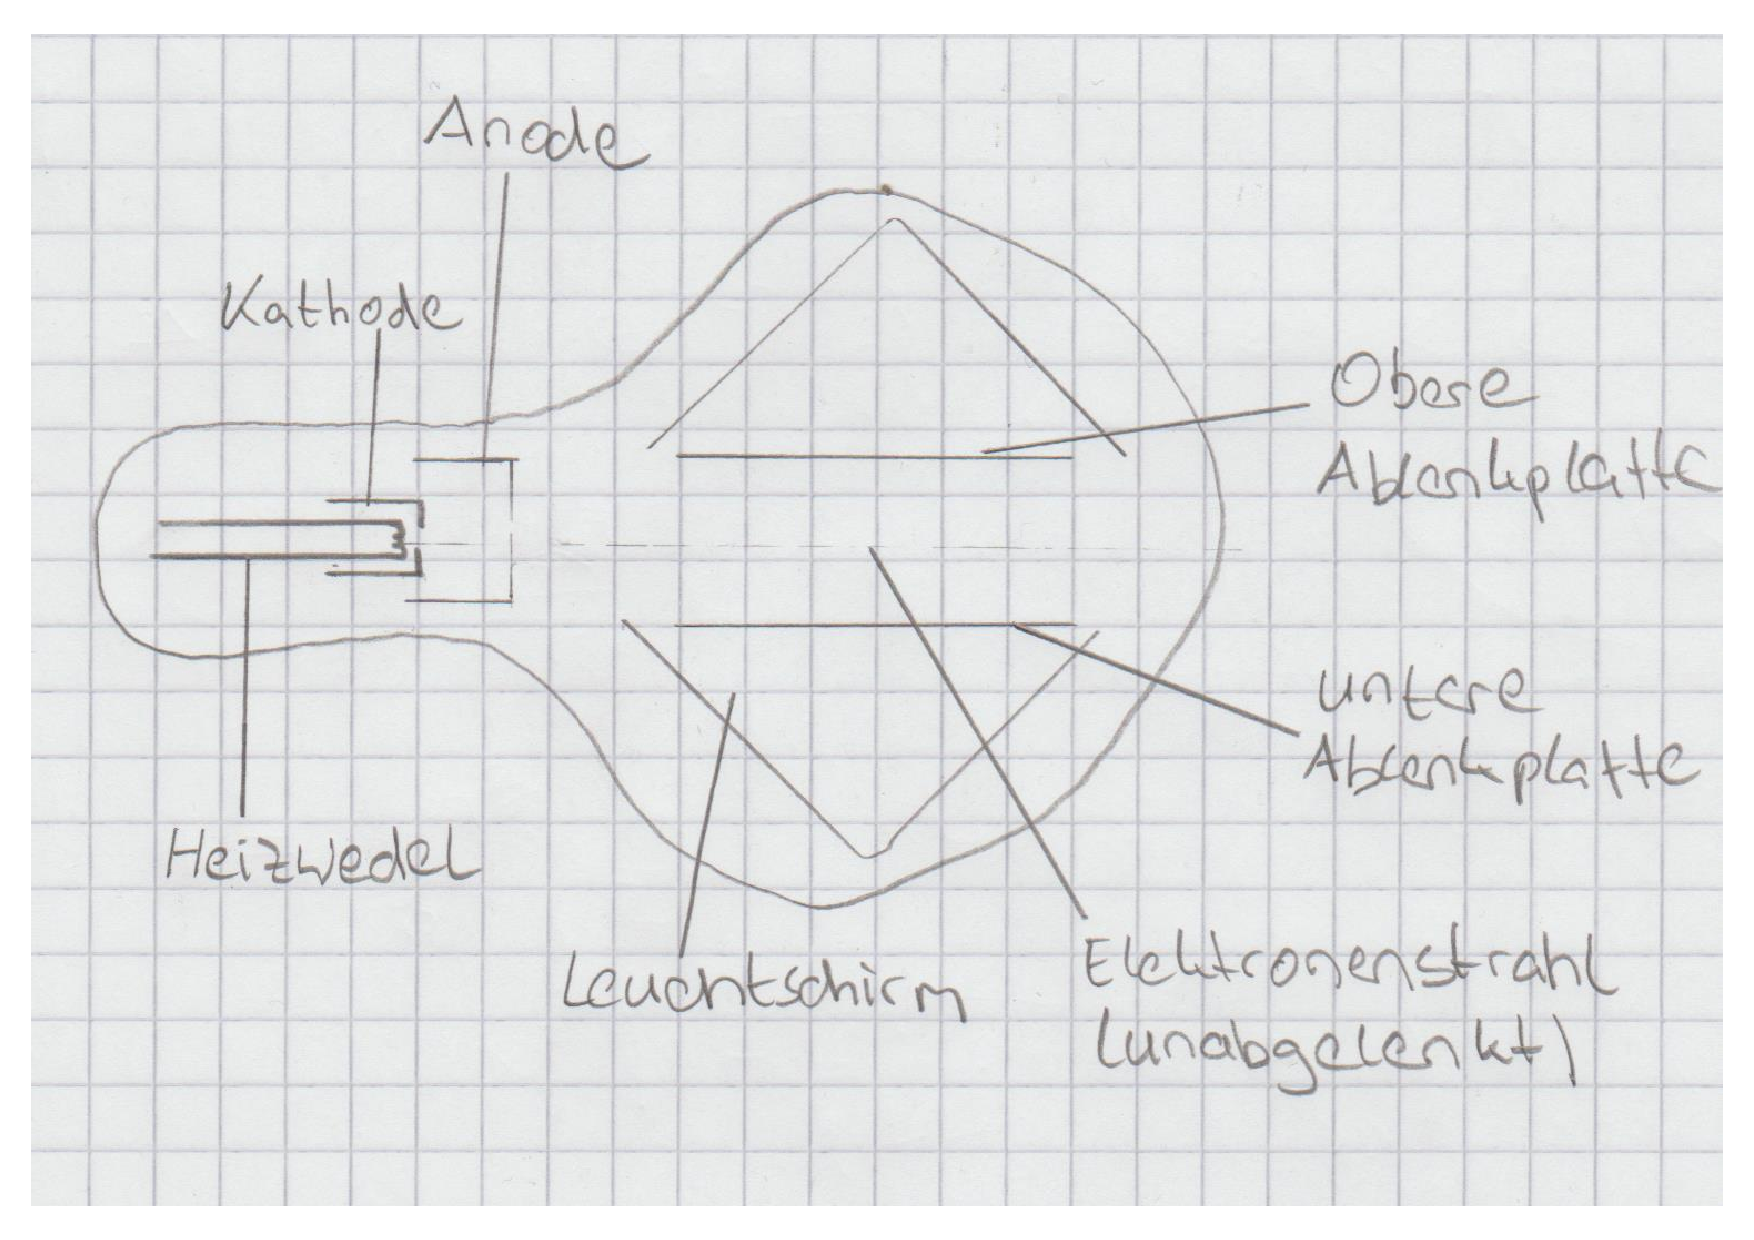
\includegraphics[width=0.7\textwidth]{./Bilder/emthomson}
\caption{Thomson-Röhre}
\end{figure}
Bei der Thomson-Röhre werden in einem evakuierten Glaskolben mithilfe eines Hochspannungsnetzgerätes, Elektronen aus einer Wolfram-Glühkathode und einer zylinderförmigen Anode beschleunigt und zu einem Elektronenstrahl gebündelt. Mithilfe eines Plattenkondensators und einer Helmholtzspule kann der Elektronenstrahl elektrostatisch und magnetisch abgelenkt werden. Durch einen Floureszenzschirm mit mm-Raster wird die Ablenkung des Elektronenstrahls sichtbar gemacht.
\FloatBarrier

	\subsection{Messaufgaben Thomson-Röhre}
	Während des gesamten Versuches darf die Anodenspannung den Maximalwert von 4 kV und der Spulenstrom den Wert 0,9 A nicht übersteigen. \\
	Die Messungen werden in einen abgedunkelten Raum durchgeführt, damit der Elektronenstrahl besser sichtbar ist.
	\begin{enumerate}
\item Wie verhält sich der Elektronenstrahl unter Änderung der Anodenspannung und des Spulenstromes?
\item Bestimmen des Krümmungsradius r des abgelenkten Elektronenstrahls mithilfe folgender Gleichung:
\begin{align*}
r=\frac{80^2mm^2+e^2}{\sqrt{2}(80mm-e)}
\end{align*}
\item Bestimmen der magnetischen Flussdichte des Magnetfeldes durch folgende Gleichung:
\begin{align*}
B=(\frac{4}{5})^{\frac{3}{2}}*\frac{{\mu}_0*n}{R}*I=K*I
\end{align*}
Der Kalibrier-Faktor für den angegebenen Aufbau ist laut Hersteller K~=~3,5~mT/A bzw.
K~=~4,2~mT/A.
\item Bestimmen von e/m aus Spannung, Magnetfeld und Radius.
\item Aufnehmen von Werteparren I und U bei konstanten Radius r.
\item Fehlerbetrachtung für der Messungen.
\item Graphisches bestimmen von e/m mit Berücksichtigung der Fehler.
\end{enumerate}
	
	\subsection{Versuchsaufbau Doppelstrahlröhre}
	Benötigte Geräte:
	\begin{itemize}
\item Doppelstrahlröhre in Helmholtzspule
\item Netzgerät
\item Multimeter als Spannungsmesser
\item Multimeter als Strommesser
\end{itemize}
\begin{figure}[h]
\centering
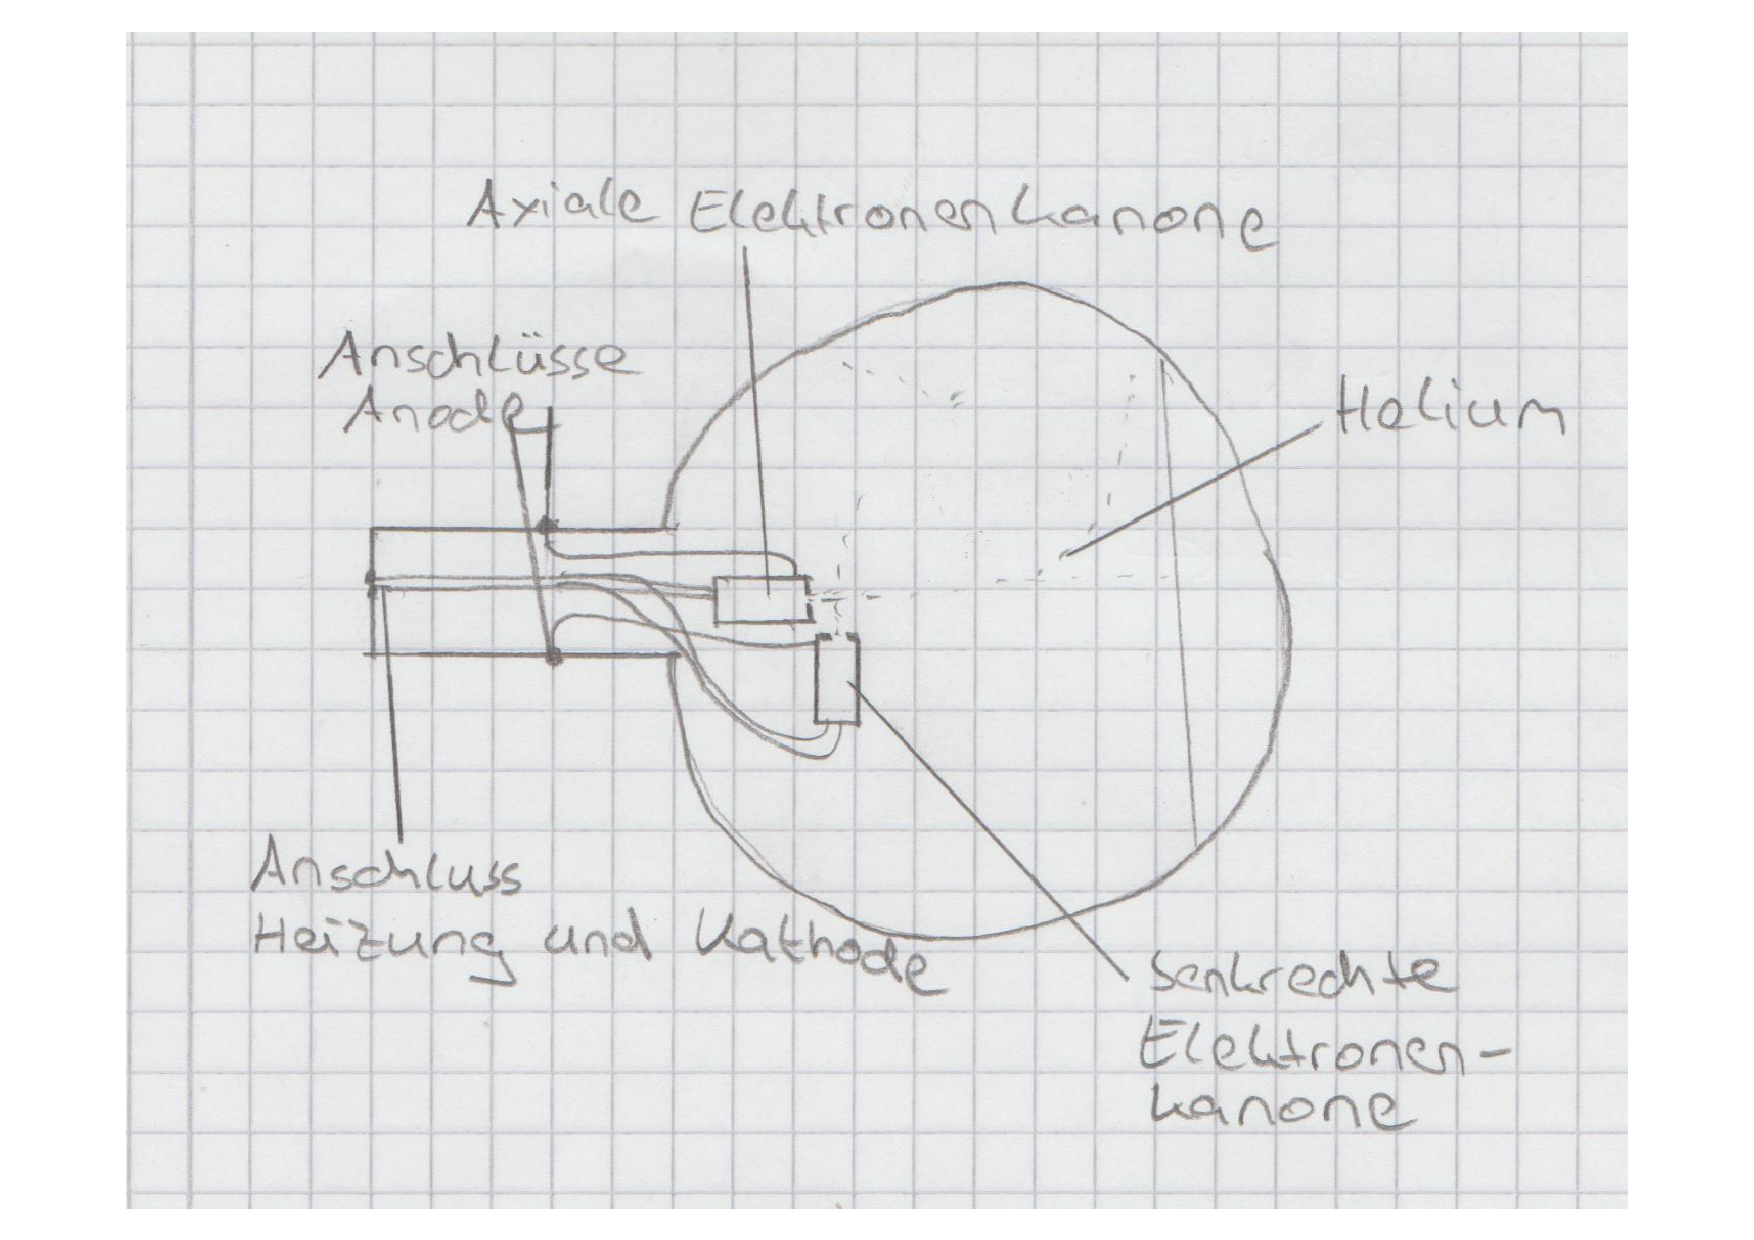
\includegraphics[width=0.7\textwidth]{./Bilder/emdoppel}
\caption{Doppelstrahlröhre}
\end{figure}
Eine Doppelstrahlröhre ist eine mit Helium befüllte, teilevakuierte, Röhre mit tangentialer und axialer Elektronenkanone und je einer indirekt beheizten Oxid-Kathode. Die senkrecht zueinander
angeordneten Elektronenstrahlen ermöglichen eine gemeinsame Ablenkplatte für beide Elektronenkanonen. In dem Glaskörper können sich fast alle Elektronen im Elektronenbündel ungehindert bewegen. 
Durch Zusammenstöße mit Heliumatomen wird die Elektronenbahn aufgrund der Anregung sichtbar.

\FloatBarrier
	\subsection{Messaufgaben Doppelstrahlröhre}
Während des gesamten Versuches darf die Plattenspanung den Maximalwert von 45 V und der Spulenstrom den Wert 0,4 A nicht übersteigen.
	 \begin{enumerate}
	 \item Berechnen von e/m durch Messung des Radius, der Stromstärke und der Plattenspannung mithilfe Formel (4).
	 Das
Magnetfeld lässt sich durch die Helmholtz-Anordnung über folgende Beziehung bestimmen:
\begin{align*}
B^2=17,39*10^{-6}*{I_H}^2
\end{align*}
	 \item Berechen e/m für drei weitere Radien bei konstanter Plattenspannung.
	 \item Fehlerbetrachtung der Messung.
	 \end{enumerate}
	
    
	
	
	
	
	\end{document}
	
